\documentclass[12pt]{extarticle}
%Some packages I commonly use.
\usepackage[portuguese]{babel}
\usepackage{graphicx}
\usepackage{framed}
\usepackage[normalem]{ulem}
\usepackage{amsmath}
\usepackage{amsthm}
\usepackage{amssymb}
\usepackage{amsfonts}
\usepackage{enumerate}
\usepackage[utf8]{inputenc}
\usepackage{float}
\usepackage{gensymb}
\usepackage[top=1 in,bottom=1in, left=1 in, right=1 in]{geometry}
\usepackage{multirow}
\usepackage{caption}
\usepackage{subcaption}
\usepackage[utf8]{inputenc}


%A bunch of definitions that make my life easier
\newcommand{\matlab}{{\sc Matlab} }
\newcommand{\cvec}[1]{{\mathbf #1}}
\newcommand{\rvec}[1]{\vec{\mathbf #1}}
\newcommand{\ihat}{\hat{\textbf{\i}}}
\newcommand{\jhat}{\hat{\textbf{\j}}}
\newcommand{\khat}{\hat{\textbf{k}}}
\newcommand{\minor}{{\rm minor}}
\newcommand{\trace}{{\rm trace}}
\newcommand{\spn}{{\rm Span}}
\newcommand{\rem}{{\rm rem}}
\newcommand{\ran}{{\rm range}}
\newcommand{\range}{{\rm range}}
\newcommand{\mdiv}{{\rm div}}
\newcommand{\proj}{{\rm proj}}
\newcommand{\R}{\mathbb{R}}
\newcommand{\N}{\mathbb{N}}
\newcommand{\Q}{\mathbb{Q}}
\newcommand{\Z}{\mathbb{Z}}
\newcommand{\<}{\langle}
\renewcommand{\>}{\rangle}
\renewcommand{\emptyset}{\varnothing}
\newcommand{\attn}[1]{\textbf{#1}}
\theoremstyle{definition}
\newtheorem{theorem}{Theorem}
\newtheorem{corollary}{Corollary}
\newtheorem*{definition}{Definition}
\newtheorem*{example}{Example}
\newtheorem*{note}{Note}
\newtheorem{exercise}{Exercise}
\newcommand{\bproof}{\bigskip {\bf Proof. }}
\newcommand{\eproof}{\hfill\qedsymbol}
\newcommand{\Disp}{\displaystyle}
\newcommand{\qe}{\hfill\(\bigtriangledown\)}
\setlength{\columnseprule}{1 pt}
\usepackage[utf8]{inputenc}

\title{Aula 23 - Gravitação}
\author{Felipe Salvador}
\date{Atualizado em \today}

\begin{document}

\maketitle

\section{Introdução}
A Gravitação é uma área dentro da \textbf{Astronomia} que estuda sobre os processos, mecanismos e movimentos de estrelas e planetas devido à força da gravidade. Esses estudos começaram lá no século XVII com o astronômo alemão Johannes Kepler e com o físico/astrônomo italiano Galileu Galilei, perseguido pela Inquisição da Igreja.

Ambos perceberam que a Terra não era o centro do Sistema Solar (modelo geocêntrico) que a Igreja afirmava, mas que o Sol era o centro do Sistema (modelo heliocêntrico). Ou seja, a Terra era que orbitava ao redor do Sol, não o contrário. Isso foi o que engatilhou a perseguição da Igreja contra Galilei, que resultou numa confissão forçada de Galilei dizendo que o que ele descobriu era uma farsa.

Os primeiros grandes resultados sobre a órbita dos planetas ao redor do Sol foram as \textbf{Leis de Kepler:}

\section{Leis de Kepler}
Ao todo, as Leis de Kepler são 3:
\begin{enumerate}
    \item \textbf{1$^a$ Lei} - Lei das Órbitas;
    \item \textbf{2$^a$ Lei} - Lei das Áreas;
    \item \textbf{3$^a$ Lei} - Lei dos Períodos;
\end{enumerate}

\subsection{1$^a$ Lei - Lei das Órbitas}
O enunciado dessa Lei é:
\begin{quote}
    A órbita dos planetas é sobre uma elipse em que o Sol está em um dos focos da elipse
\end{quote}

Uma questão importante dessa Lei é que o movimento dos planetas é bem definido e pode ser visto na figura a seguir:
\begin{figure}[H]
    \centering
    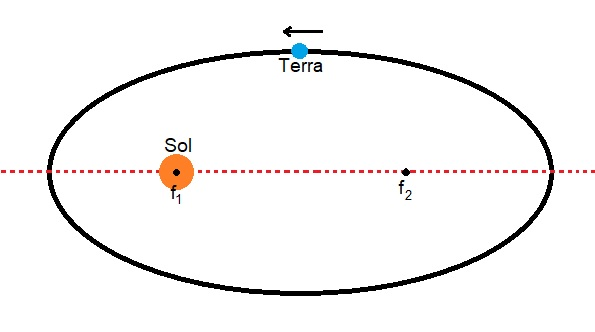
\includegraphics[width=0.6\textwidth]{primeira_lei.jpg}
    \caption{Ilustração do formato da órbita dos planetas ao redor do Sol. Os pontos $f_1,\,f_2$ são chamados de 'focos da elipse', em que o Sol estará sobre um desses focos.}
    \label{fig:primeira_lei}
\end{figure}
2 outras questões importantes: \textbf{O ponto da órbita mais distante do Sol é chamado de Afélio e o ponto da órbita mais próximo do Sol é chamado de Periélio.} No caso de satélites orbitando os planetas, como é o caso da Lua, os pontos são chamados de \textbf{Apogeu e Perigeu}.

Uma parâmetro de interesse das órbitas é chamado de excentricidade ($\epsilon$) - é uma quantidade que me diz o quão "achatada" a elipse está em comparação com um círculo. \textbf{Se a excentricidade for zero ($\epsilon=0$), a elipse se torna um círculo.}
\begin{figure}[H]
    \centering
    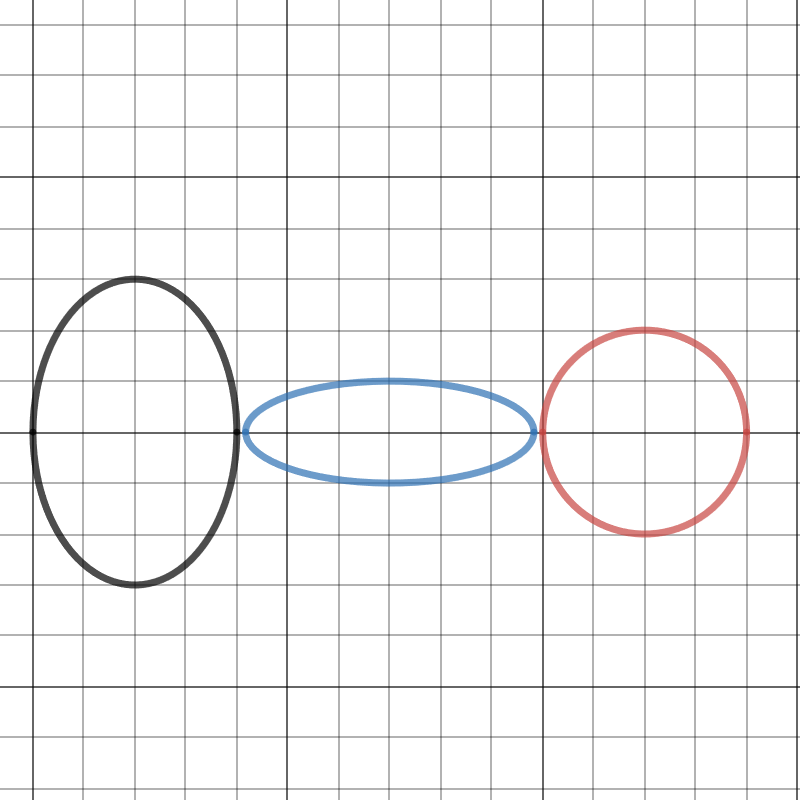
\includegraphics[width=0.4\textwidth]{eccentricity.png}
    \caption{Exemplos de elipses com diferentes excentricidades: A elipse em preto com excentricidade é de 0.74, a elipse em azul tem excentricidade 0.86 e a elipse em vermelho tem excentricidade 0 (perceba que é um circulo)}
    \label{fig:excentricidade}
\end{figure}

Para elipses, a excentricidade é dada por:
\begin{equation}
    \epsilon = \sqrt{1- \frac{b^2}{a^2}}
\end{equation}
\noindent em que 'b' é o raio menor da elipse e 'a' é o raio maior.
\begin{figure}[H]
    \centering
    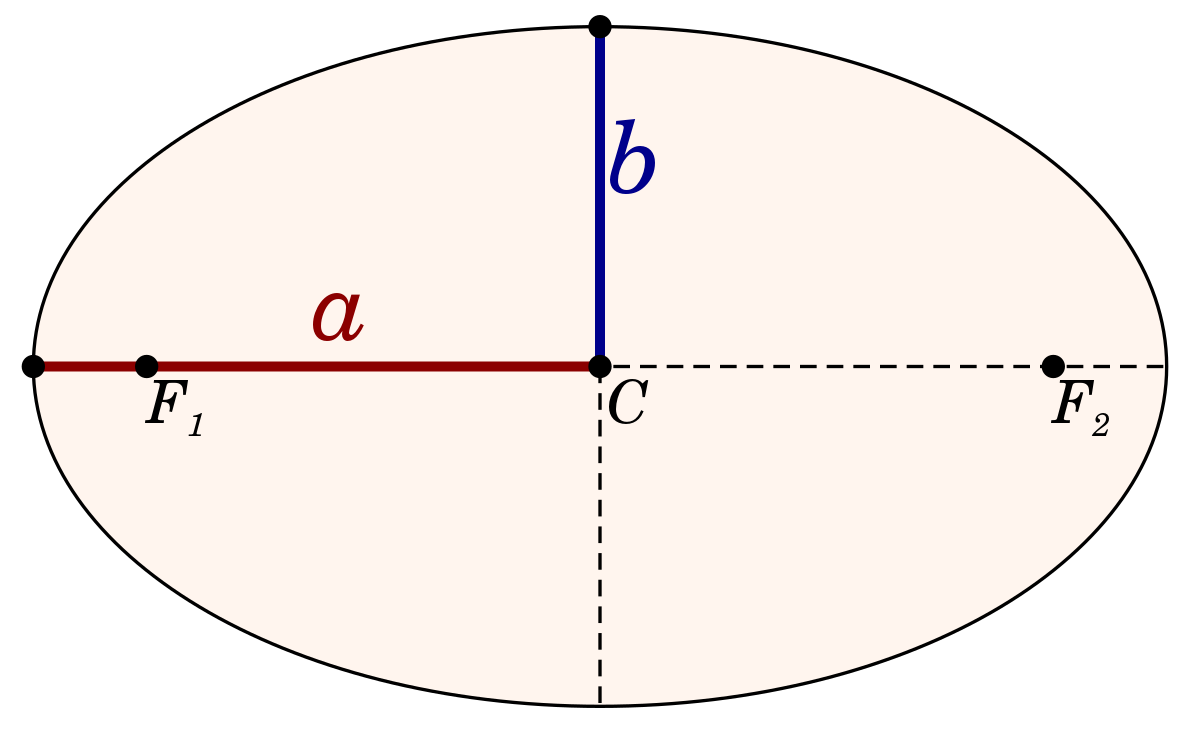
\includegraphics[width=0.6\textwidth]{1200px-Ellipse_semi-major_and_minor_axes.svg.png}
    \caption{Ilustração dos raios menor e maior de uma elipse}
    \label{fig:minor_major_radius}
\end{figure}

\subsection{$2^a$ Lei de Kepler - Lei das Áreas}
O enunciado da 2$^a$ Lei é:
\begin{quote}
    A linha que liga o Sol ao planeta varre áreas iguais em intervalos de tempo iguais.
\end{quote}

A ilustração dessa Segunda Lei é a seguinte:
\begin{figure}[H]
    \centering
    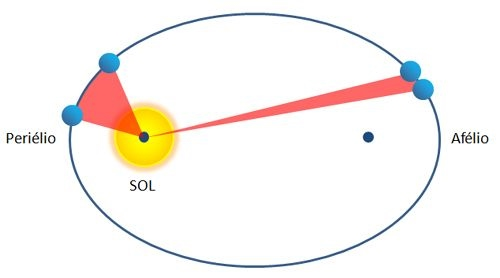
\includegraphics[width=0.6\textwidth]{segunda_lei.jpg}
    \caption{Ilutração da Segunda Lei de Kepler - As áreas que a linha entre o planeta e o Sol varre são as mesmas para um período de tempo igual}
    \label{fig:2nd_law}
\end{figure}

Essa Lei traz um sentido bem especial -  a velocidade de órbita não é necessariamente constante. Como as áreas tem que ser iguais, então quando o planeta está perto de uma estrela, a velocidade de orbita dele é grande para ele consiga varrer essa área. Porém, quando ele está longe, a velocidade da órbita é pequena. 

Dessa forma, os planetas passam por um movimento acelerado quando eles estão no ponto em que se aproximam da estrela e passam por um movimento retardado quando eles estão se afastando da estrela.

A diferença de velocidade é dada pela seguinte relação:
\begin{equation}
    v_p\,r_p = v_a\,r_a
\end{equation}
\noindent em que $v_p,\,v_a$ são as velocidades no periélio e no afélio, respectivamente, e $r_p,\,r_a$ são a distância entre o planeta e a estrela no periélio e no afélio, respectivamente.

\subsection{$3^a$ Lei de Kepler - Lei dos Períodos}
O enunciado da $3^a$ Lei é:
\begin{quote}
    A razão entre o quadrado do período de translação e o cubo do raio maior da orbita é uma constante.
\end{quote}
Em matematiquês:
\begin{equation}
    \frac{T^2}{b^3} = k
\end{equation}
\noindent em que $T$ é o período de translação, ou seja, quanto tempo demorar para dar uma volta na órbita,  $b$ é o raio maior da elipse em que o planeta orbita e $k$ é um número.

Para 2 planetas que orbitam uma mesma estrela:
\begin{equation}
    \frac{T_A^2}{b_A^3} = \frac{T_B^2}{b_B^3}
\end{equation}

\section{Lei da Gravitação de Newton}
Junto com o seu trabalho sobre Mecânica e as Leis de Newton, em 1687, Isaac Newton desenvolveu a \textbf{Lei da Gravitação Universal}, que descrevia a Força da gravidade entre 2 corpos:
\begin{equation}
    F_{g} = \frac{G\,M\,m}{d^2}
\end{equation}
\noindent em que '$M,\,m$' são as massas dos corpos envolvidos, '$d$' é a distância entre os corpos e '$G$' é a constante gravitacional ($G\approx 6,67\,\times 10^{-11} m^3\,kg^{-1}\,s^{-2}$)

\begin{figure}[H]
    \centering
    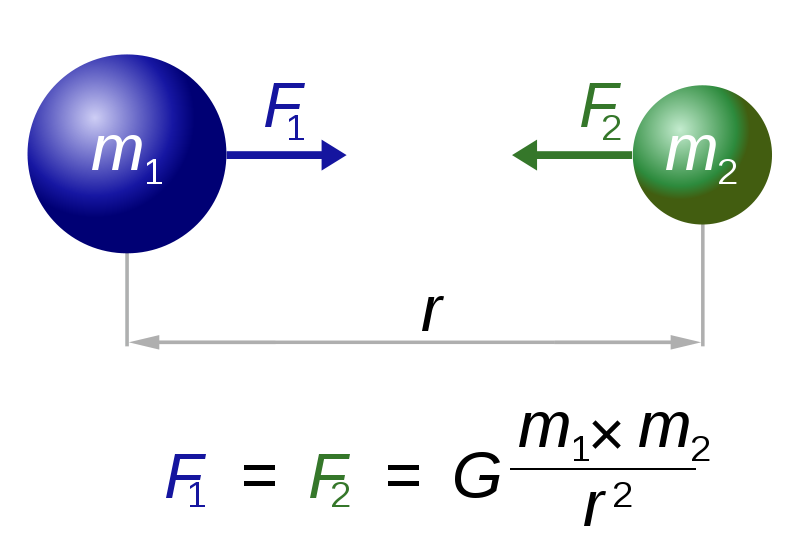
\includegraphics[width=0.4\textwidth]{800px-NewtonsLawOfUniversalGravitation.svg.png}
    \caption{Ilustração da Força gravitacional entre os corpos. Perceba que o módulo da força que cada corpo age sobre o outro é o mesmo.}
    \label{fig:newton_gravitational}
\end{figure}

\subsection{Campo Gravitacional}
Um conceito de grande utilidade na Física é o conceito de Campo. Assim como no caso da eletricidade e do magnetismo, o campo gravitacional carrega consigo o comportamento da força peso (direção e proporcionalidade), para que depois, com a massa que for interagir, possamos determinar o sentido e o módulo da força peso. 

Da mesma forma que fizemos para a eletricidade e magnetismo, o campo gravitacional($g$) é deduzido assim:
\begin{equation}
    F_{g} = \frac{G\,M\,m}{d^2}  = \frac{G\,M}{d^2}\,m = g\,m
\end{equation}
\noindent em que $g = \frac{G\,M}{d^2}$. A unidade de $g$ é $\frac{N}{kg}$ ou $m/s^2$.

Para o caso da força da gravidade gerada na Terra na superfície dela: $M_{terra} = 5.97\times10^{24}\,kg$ e $r_{terra} = 6,37\times10^6\,m$, logo o campo gravitacional:
\begin{equation}
    g = \frac{G\,M_{terra}}{d_{terra}^2} = \frac{6,67\times10^{-11}\,5,97\times10^{24}}{(6,37\times10^{6})^2} \approx 9,8\,m/s^2 
\end{equation}
\noindent que é a aceleração da gravidade que temos usado nos exercícios.

\subsection{Velocidade de Órbita}
A força gravitacional é a força que mantém os corpos (planetas, satélites) sobre a órbita. Com isso, ela faz o papel de força centrípeta do movimento circular que os planetas fazem. \footnote{Apesar dos planetas orbitarem numa elipse, para o nosso Sistema Solar, a órbita da maioria dos planetas é quase circular (excentricidade bem próxima de 0), exceto para o caso de Mercúrio, cuja órbita tem excentricidade de 0,22.} 

\begin{figure}[H]
    \centering
    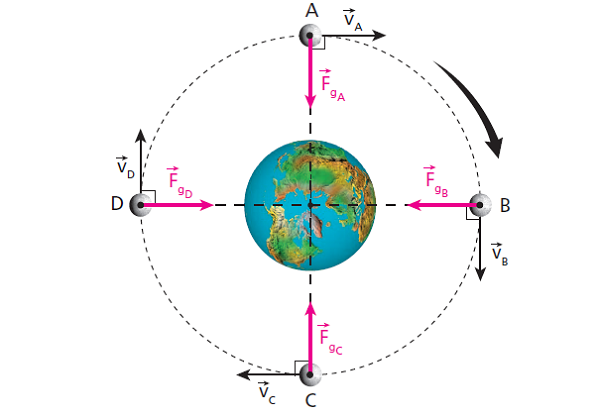
\includegraphics[width=0.6\textwidth]{centripetal_force_gravitational.png}
    \caption{Diagrama de forças no caso de um satélite orbitando a Terra. Perceba que a força sempre é direção à Terra e sempre está perpendicular ao movimento do satélite}
    \label{fig:centripetal}
\end{figure}
Assim, podemos tratar a força gravitacional como força centrípeta e usar sua fórmula:
\begin{equation}
    F_g = F_c \implies \frac{G\,M\,m}{r_{orb}^2} = \frac{m\,v_{orb}^2}{r_{orb}} \implies \boxed{v_{orb} = \sqrt{\frac{GM}{r_{orb}}}}
\end{equation}

Com isso, conforme mais longe do corpo que eu estiver orbitando ao redor, mais lento eu estarei fazendo a órbita. Porém, quanto mais próximo do corpo, mais rápido eu estarei se movimentando.

Para o caso da Terra ao redor do Sol, sabendo que a massa do Sol é: $M=1,989\times10^{30}\,kg$ e a distância Terra-Sol: $r_{orb} = 1,5\times10^{11}\,m$ ou $1\,UA$ (UA - Unidade Astronômica):
\begin{equation}
    v_{terra}=\sqrt{\frac{6,67\times10^{-11}\,1,989\times10^{30}}{1,5\times10^{11}}}= \sqrt{8,84\times10^{8}} \approx 29732,1\,km/s
\end{equation}
\subsection{Período da Órbita}
Podemos também calcular o período da órbita - é o tempo que um corpo demora para dar uma volta ao redor da estrela. Partindo da velocidade de órbita:
\begin{equation}
    v_{orb} = \frac{\Delta S}{\Delta t} = \frac{2\pi r_{orb}}{T}
\end{equation}
\noindent em que foi suposto que a órbita seja aproximadamente circular. Se substituirmos na fórmula da velocidade de órbita:
\begin{equation}
    v_{orb} = \sqrt{\frac{GM}{r_{orb}}} \implies v_{orb}^2 = \frac{GM}{r_{orb}} \implies \frac{4\pi^2\,r_{orb}^2}{T^2} = \frac{GM}{r_{orb}} \implies \frac{T^2}{r_{orb}^3} = \frac{4\pi^2}{GM}
\end{equation}
Perceba que o lado esquerdo é o mesmo lado esquerdo da Terceira Lei de Kepler. Então, a constante da Lei de Kepler é dada por:
\begin{equation}
    k = \frac{4\pi^2}{GM}
\end{equation}
Voltando na equação (11), passando o $r_{orb}^3$ para o outro lado e tirando a raiz quadrada:
\begin{equation}
    T = \sqrt{\frac{4\pi^2\,r_{orb}^3}{GM}}
\end{equation}
Fazendo as contas para a Terra orbitando ao redor do Sol: $M=1,989\times10^{30}\,kg$ e a distância Terra-Sol: $r_{orb} = 1,5\times10^{11}\,m$:
\begin{equation}
    T_{terra} = \sqrt{\frac{4\pi^2(1,5\times10^{11})^3}{6,67\times10^{-11}1,989\times10^{30}}} \approx 31.691.036\,s \approx 366,79 \, dias
\end{equation}
A diferença para o nosso ano (365,24 dias) é de aproximadamente de $\pm 1$ dia. Ou seja, o erro que cometemos ao supor que a Terra faça uma órbita circular foi de $\approx 0,004\%$.

\section{Energia Potencial Gravitacional}
Já vimos o conceito de energia potencial e sabemos que podemos definir a energia potencial para o caso gravitacional. Nesse caso, a energia potencial gravitacional ($E_{pg}$) é:
\begin{equation}
    E_{pg} = - \frac{G\,M\,m}{d}
\end{equation}
\noindent em que 'G' é a constante gravitacional, '$M,\,m$' são as massas dos corpos e 'd' é a distância entre eles. \textbf{Perceba que essa energia é negativa.} Conforme maior for as massas ou mais perto elas estejam entre si, a energia será cada vez mais negativa. 

Com isso, podemos calcular a chamada velocidade de escape da Terra.
\subsection{Velocidade de Escape}
A velocidade de escape é calculada a partir do seguinte exercício: \textbf{Supondo um corpo que não tenha um motor, qual deve ser a velocidade inicial dele para ele consiga escapar da Terra?}
Bem essa pergunta pode ser respondida a partir do princípio de conservação de energia. Supondo que não haja atrito nem resistência do ar, a conservação de energia me diz o seguinte:
\begin{equation}
    (E_t)_1=(E_t)_2 \implies (E_{pg})_1 + (E_c)_1 = (E_{pg})_2 + (E_c)_2
\end{equation}
Dizemos que um objeto escapou da atração gravitacional da Terra quando a energia potencial relacionada a ele for 0. Para o cálculo da velocidade de escape, queremos a velocidade mínima em que o objeto consegue escapar, ou seja, quando o objeto conseguir finalmente se desfazer da atração gravitacional, ele pare (energia cinética 0). Assim:
\begin{equation}
    (E_{pg})_1 + (E_c)_1 = 0+0=0
\end{equation}
Substituindo as fórmulas, supondo que ele saia da superfície da Terra ao nível do mar:
\begin{equation}
    -\frac{G\,M\,m}{R} + \frac{mv^2}{2}=0 \implies v^2 = \frac{2GM}{R}
\end{equation}
Substituindo os valores da massa da Terra e o raio da terra: $M=5,97\times10^{24}\,kg$ e $R=6,37\times10^6\,m$:
\begin{equation}
    v_e = \sqrt{\frac{2GM}{R}} \implies v =\sqrt{\frac{2*6,67\times10^{-11}\,5,97\times10^{24}}{6,37\times10^6}} \approx 11,2 km/s
\end{equation}

Esse valor difere muito da real velocidade de escape: $v_e= 11,186\,km/s$, porque a resistência do ar freia muito o corpo que está tentando sair da terra. Essa diferença é bem grande, uma vez que, a força da resistência do ar depende com o quadrado da velocidade do corpo em movimento. Ou seja, conforme a velocidade do corpo tentando sair da Terra aumenta, a força da resistência do ar aumenta muito mais. \footnote{Força de resistência do ar: $F = \frac{1}{2}C\,\rho\,A\,v^2$, em que $C,\,\rho,\,A$ são uma constante de arrasto (adimensional), densidade volumétrica de massa do ar e a área de contato frontal do corpo com o ar.}

\section{Lua e Eclipses}
A Lua é o único satélite natural que a Terra possui. Ao todo a Lua passa por 4 fases que duram 28 dias - 1 mês lunar:
\begin{itemize}
    \item Lua Cheia
    \item Quarto Minguante
    \item Lua Nova
    \item Quarto Crescente
\end{itemize}
\begin{figure}[H]
    \centering
    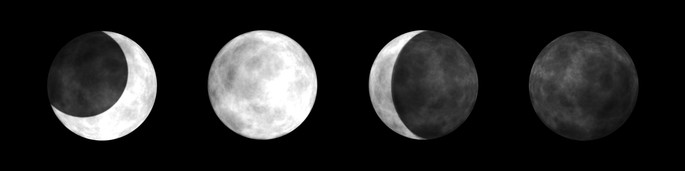
\includegraphics[width=0.7\textwidth]{fasesdaluahemisferiosul-cke.jpg}
    \caption{As fases da Lua}
    \label{fig:moon_phases}
\end{figure}

A Lua também faz parte de raros eventos astronômicos: os eclipses solar e lunar. Os eclipses são eventos raros, pois a Terra orbita ao redor do Sol num plano diferente do que a Lua orbita a Terra. Os eclipses acontecem quando há um alinhamento entre os 3 corpos. Logo, os eclipses são caracterizados por:
\begin{itemize}
    \item \textbf{Eclipse Solar} - quando há um alinhamento Sol-Lua-Terra, de forma que a Lua faz uma sombra numa região da Terra durante o dia.
    
    \begin{figure}[H]
        \centering
        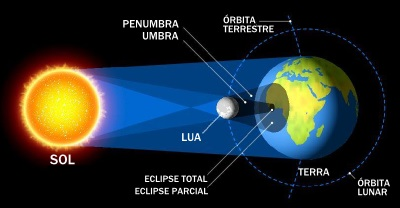
\includegraphics[width=0.8\textwidth]{esquema-do-eclipse-solar.jpg}
        \caption{Eclipse Solar e os nomes das sombras}
        \label{fig:solar_eclipse}
    \end{figure}
    
    \item \textbf{Eclipse Lunar} - é quando há um alinhamento Sol-Terra-Lua, de forma que a Terra faz sombra na Lua:
    \begin{figure}[H]
        \centering
        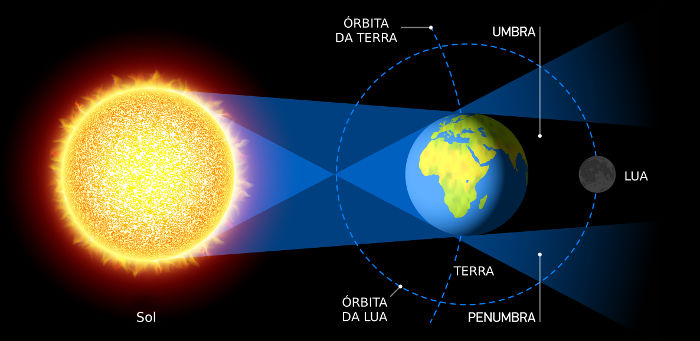
\includegraphics[width=0.8\textwidth]{esquema-eclipse-lunar.jpg}
        \caption{Eclipse Lunar e os nomes das sombras}
        \label{fig:lunar_eclipse}
    \end{figure}
\end{itemize}
\end{document}
